\hypertarget{mvt_8h}{
\section{mvt.h File Reference}
\label{mvt_8h}\index{mvt.h@{mvt.h}}
}


This graph shows which files directly or indirectly include this file:\nopagebreak
\begin{figure}[H]
\begin{center}
\leavevmode
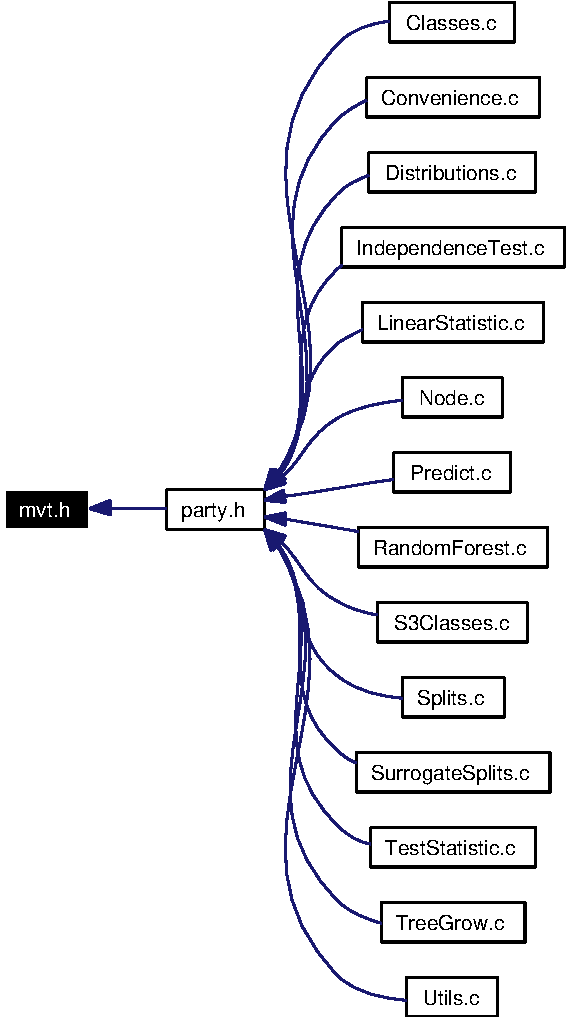
\includegraphics[width=420pt]{mvt_8h__dep__incl}
\end{center}
\end{figure}
\subsection*{Functions}
\begin{CompactItemize}
\item 
void F77\_\-NAME() \hyperlink{mvt_8h_2a7ae850a24d2fe1a610ca397d6871c7}{mvtdst} (int $\ast$n, int $\ast$nu, double $\ast$lower, double $\ast$upper, int $\ast$infin, double $\ast$corr, double $\ast$delta, int $\ast$maxpts, double $\ast$abseps, double $\ast$releps, double $\ast$error, double $\ast$value, int $\ast$inform)
\end{CompactItemize}


\subsection{Function Documentation}
\hypertarget{mvt_8h_2a7ae850a24d2fe1a610ca397d6871c7}{
\index{mvt.h@{mvt.h}!mvtdst@{mvtdst}}
\index{mvtdst@{mvtdst}!mvt.h@{mvt.h}}
\subsubsection[{mvtdst}]{\setlength{\rightskip}{0pt plus 5cm}void F77\_\-NAME() mvtdst (int $\ast$ {\em n}, \/  int $\ast$ {\em nu}, \/  double $\ast$ {\em lower}, \/  double $\ast$ {\em upper}, \/  int $\ast$ {\em infin}, \/  double $\ast$ {\em corr}, \/  double $\ast$ {\em delta}, \/  int $\ast$ {\em maxpts}, \/  double $\ast$ {\em abseps}, \/  double $\ast$ {\em releps}, \/  double $\ast$ {\em error}, \/  double $\ast$ {\em value}, \/  int $\ast$ {\em inform})}}
\label{mvt_8h_2a7ae850a24d2fe1a610ca397d6871c7}




Referenced by C\_\-maxabsConditionalPvalue().